%!TEX TS-program = xelatex
%!TEX options = -aux-directory=Debug -shell-escape -file-line-error -interaction=nonstopmode -halt-on-error -synctex=1 "%DOC%"
\documentclass{article}
\input{LaTeX-Submodule/template.tex}

% Additional packages & macros
\usepackage{changepage} % Modify page width
\usepackage{multicol} % Use multiple columns
\usepackage[explicit]{titlesec} % Modify section heading styles
\setitemize{leftmargin=*,topsep=1ex,partopsep=0ex,itemsep=-1ex,partopsep=0ex,parsep=1ex}
\setlist{leftmargin=*,topsep=1ex,partopsep=0ex,itemsep=-1ex,partopsep=0ex,parsep=1ex}

\titleformat{\section}{\raggedright\normalfont\bfseries}{}{0em}{#1}
\titleformat{\subsection}{\raggedright\normalfont\small\bfseries}{}{0em}{#1}

\usepackage{appendix}
\usepackage{subcaption}
\usepackage{algorithm}
\usepackage{algpseudocode}
\usepackage{algorithmicx}
\usepackage{nicematrix}

\DeclareMathOperator{\argmin}{arg\, min}

%% A4 page
\geometry{
	a4paper,
	margin = 10mm
}

%% Hide horizontal rule
\renewcommand{\headrulewidth}{0pt}
\fancyhead{}

%% Hide page numbers
\pagenumbering{gobble}

%% Multi-columns setup
\setlength\columnsep{4pt}

%% Paragraph setup
\setlength\parindent{0pt}
\setlength\parskip{0pt}

% Metadata for README
\newcommand{\unitName}{Computational Mathematics 2}
\newcommand{\unitTime}{Semester 1, 2024}
\newcommand{\unitCoordinator}{Dr Elliot Carr}
\newcommand{\documentAuthors}{Tarang Janawalkar}

%% Copyright
\usepackage[
    type={CC},
    modifier={by-nc-sa},
    version={4.0},
    imagewidth={5em},
    hyphenation={raggedright}
]{doclicense}

\begin{document}
% Modify spacing
\titlespacing*\section{0pt}{1ex}{1ex}
\titlespacing*\subsection{0pt}{1ex}{1ex}
%
\setlength\abovecaptionskip{8pt}
\setlength\belowcaptionskip{-15pt}
\setlength\textfloatsep{0pt}
%
\setlength\abovedisplayskip{1pt}
\setlength\belowdisplayskip{1pt}
\begin{figure}[H]
    \centering
    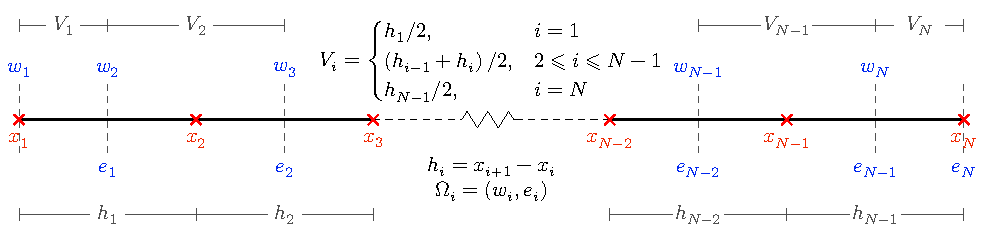
\includegraphics[width = 0.8\linewidth]{figures/1d-fvm-exam.pdf}
\end{figure}
\begin{minipage}[t]{126.1962963mm}
    \begin{align*}
        u\left( w_i,\: t \right)           & = \left( 1 - \sigma \right) u_{i-1} + \sigma u_i & \pdv{u}!{x}\left( w_i,\: t \right) & = \left( u_i - u_{i-1} \right) / h_{i-1} &  & \text{(west node)}  \\
        u\left( e_i,\: t \right)           & = \left( 1 - \sigma \right) u_i + \sigma u_{i+1} & \pdv{u}!{x}\left( e_i,\: t \right) & = \left( u_{i+1} - u_i \right) / h_i     &  & \text{(east node)}  \\
        \pdv{u}!{x}\left( w_1,\: t \right) & = \pdv{u}!{x}\left( 0,\: t \right)               & \pdv{u}!{x}\left( e_1,\: t \right) & = \left( u_2 - u_1 \right) / h_1         &  & \text{(node 1)}     \\
        \pdv{u}!{x}\left( w_N,\: t \right) & = \left( u_N - u_{N-1} \right) / h_{N-1}         & \pdv{u}!{x}\left( e_N,\: t \right) & = \pdv{u}!{x}\left( L,\: t \right)       &  & \text{(node \(N\))}
    \end{align*}
    \(D\left( u\left( x_i,\: t \right) \right) = D\left( u_i \right)\),
    \(D\left( u\left( w_i,\: t \right) \right) = \frac{D\left( u_{i-1} \right) + D\left( u_i \right)}{2}\),
    \(D\left( u\left( e_i,\: t \right) \right) = \frac{D\left( u_i \right) + D\left( u_{i+1} \right)}{2}\)
    \section{Time Discretisation (integrate between \texorpdfstring{\(t_n\)}{tn} and \texorpdfstring{\(t_{n+1}\)}{tn+1})}
    \begin{gather*}
        \left( \symbf{I} - \fdif{t} \theta_1 \symbf{A} \right) \symbf{u}^{\left( n+1 \right)} = \left[ \symbf{I} + \fdif{t} \left( 1 - \theta_1 \right) \symbf{A} \right] \symbf{u}^{\left( n \right)} + \fdif{t} \left[ \symbf{b}_1 + \left( 1 - \theta_2 \right) \symbf{b}_2^{\left( n \right)} + \theta_2 \symbf{b}_2^{\left( n+1 \right)} \right] \\
        \text{using } {\textstyle\int_{t_n}^{t_{n+1}}} f\left( t \right) \odif{t} \approx \fdif{t} \left[ \left( 1 - \theta \right) f\left( t_n \right) + \theta f\left( t_{n+1} \right) \right],\: \tilde{\symbf{A}} \symbf{u}^{\left( n+1 \right)} = \tilde{\symbf{B}} \symbf{u}^{\left( n \right)} + \tilde{\symbf{c}} = \tilde{\symbf{b}}
    \end{gather*}
    \textbf{FE} (\(\theta_1 = \theta_2 = 0\)), \textbf{BE} (\(\theta_1 = \theta_2 = 1\)), \textbf{C-N} (\(\theta_1 = \theta_2 = \frac{1}{2}\)).
    \textbf{Dirichlet BCs} replace row of \(\tilde{\symbf{A}}\) with
    \(\symbf{e}_1\) or \(\symbf{e}_N \in \R^{1 \times N}\) and row of
    \(\tilde{\symbf{b}}\) with Dirichlet BC.
    \section{Krylov Methods}
    \begin{equation*}
        \symbf{K}_m\left( \symbf{A},\ \symbf{b} \right) = \text{span}\left\{ \symbf{b},\ \symbf{A} \symbf{b},\ \symbf{A}^2 \symbf{b},\ \ldots,\ \symbf{A}^{m-1} \symbf{b} \right\}
    \end{equation*}
    \textbf{Hessenberg factorisation}: \(\symbf{A} \symbf{Q} = \symbf{Q} \symbf{H}\)
    for \(\symbf{Q},\symbf{H} \in \R^{n \times n}\).
    Reduced factorisation: \(\symbf{A} \symbf{Q}_m = \symbf{Q}_{m+1} \bar{\symbf{H}}_m\)
    for \(\symbf{Q}_m \in \R^{n \times m}\), \(\bar{\symbf{H}}_m \in \R^{m+1 \times m}\).
    Rearrange for \(\symbf{q}_{j+1}\):
    \begin{align*}
        \symbf{q}_{j+1} & = \left( \symbf{A} \symbf{q}_j - h_{1j} \symbf{q}_1 - h_{2j} \symbf{q}_2 - \cdots - h_{jj} \symbf{q}_j \right) / h_{j+1,j} \\
                        & = \frac{1}{h_{j+1,j}} \left( \symbf{A} \symbf{q}_j - \sum_{i=1}^j h_{ij} \symbf{q}_i \right).
    \end{align*}
    \textbf{Arnoldi's method} apply Gram-Schmidt process to \(\symbf{\mathcal{K}}_m\left( \symbf{A},\ \symbf{b} \right)\). For \(\symbf{q}_{j+1}\):
    \begin{equation*}
        \symbf{q}_{j+1} = \frac{1}{\norm*{\symbf{v}_{j+1}}} \left( \symbf{A} \symbf{q}_j - \sum_{i=1}^j \left( \symbf{q}_i^\top \symbf{A} \symbf{q}_j \right) \symbf{q}_i \right),\ \symbf{A} \symbf{q}_j = \sum_{i=1}^j \left( \symbf{q}_i^\top \symbf{A} \symbf{q}_j \right) \symbf{q}_i + \norm*{\symbf{v}_{j+1}} \symbf{q}_{j+1}.
    \end{equation*}
    \begin{equation*}
        \bar{\symbf{H}}_1 =
        \begin{bmatrix}
            \symbf{q}_1^\top \symbf{A} \symbf{q}_1 \\
            \norm*{\symbf{v}_2}
        \end{bmatrix}
        ,
        \bar{\symbf{H}}_2 =
        \begin{bmatrix}
            \symbf{q}_1^\top \symbf{A} \symbf{q}_1 & \symbf{q}_1^\top \symbf{A} \symbf{q}_2 \\
            \norm*{\symbf{v}_2}                    & \symbf{q}_2^\top \symbf{A} \symbf{q}_2 \\
                                                   & \norm*{\symbf{v}_3}
        \end{bmatrix}
        , \ldots,
        \bar{\symbf{H}}_m =
        \begin{bmatrix}
            \symbf{H}_m \\
            h_{m+1,m} \symbf{e}_m^\top
        \end{bmatrix}
    \end{equation*}
    Left-multiply \(\bar{\symbf{H}}_m\) by \(\symbf{Q}_{m+1}\) to show
    \(\symbf{Q}_{m+1} \bar{\symbf{H}}_m = \symbf{Q}_m \symbf{H}_m + h_{m+1,m} \symbf{q}_{m+1} \symbf{e}_m^\top\),
    where \(\symbf{H}_m \in \R^{m \times m}\). Left-multiply this result
    by \(\symbf{Q}_m^\top\) to show \(\symbf{Q}_m^\top \symbf{A} \symbf{Q}_m = \symbf{H}_m\).
    \subsection{Sparse Linear Systems}
    \begin{itemize}
        \item Assume \(\symbf{x}^{\left( m \right)} \in
              \symbf{x}^{\left( 0 \right)} + \mathcal{K}_m\left(
              \symbf{A},\: \symbf{r}^{\left( 0 \right)} \right)\), for
              initial residual \(\symbf{r}^{\left( 0 \right)} =
              \symbf{b} - \symbf{A} \symbf{x}^{\left( 0 \right)} =
              \beta \symbf{q}_1\) where \(\symbf{q}_1\) is taken from
              the Gram-Schmidt process and \(\beta =
              \norm*{\symbf{r}^{\left( 0 \right)}}\).
        \item Solution form: \(\symbf{x}^{\left( m \right)} =
              \symbf{x}^{\left( 0 \right)} + \symbf{Q}_m \symbf{y}_m\),
              solve \(\symbf{y}_m\) using \(\symbf{r}^{\left( m
              \right)} = \symbf{b} - \symbf{A} \symbf{x}^{\left( m
              \right)} \perp \symbf{\mathcal{W}}_m\).
    \end{itemize}
    \textbf{FOM}: \(\symbf{\mathcal{W}}_m = \symbf{\mathcal{K}}_m\left( \symbf{A},\: \symbf{r}^{\left( 0 \right)} \right)\),
    \textbf{GMRES}: \(\symbf{\mathcal{W}}_m = \symbf{A} \symbf{\mathcal{K}}_m\left( \symbf{A},\: \symbf{r}^{\left( 0 \right)} \right)\).
    \subsection{Preconditioning (Jacobi: \texorpdfstring{\(\symbf{D}\)}{D}, Gauss-Seidel: \texorpdfstring{\(\symbf{D} + \symbf{L}\)}{D + L})}
    \textbf{Left preconditioning} (\(\symbf{M}^{-1} \symbf{A} \symbf{x} = \symbf{M}^{-1} \symbf{b}\) where \(\tilde{\symbf{r}}^{\left( 0 \right)} = \symbf{M}^{-1} \symbf{r}^{\left( 0 \right)}\)):
    \begin{itemize}
        \item \(\symbf{x}^{\left( m \right)} \in \symbf{x}^{\left( 0 \right)} + \mathcal{K}_m\left( \symbf{M}^{-1} \symbf{A},\: \tilde{\symbf{r}}^{\left( 0 \right)} \right)\),
              with \(\symbf{q}_1 = \tilde{\symbf{r}}^{\left( 0 \right)} /
              \beta\) for \(\beta = \norm*{\tilde{\symbf{r}}^{\left( 0
              \right)}}\).
        \item Arnoldi decomposition: \(\left( \symbf{M}^{-1} \symbf{A} \right)
              \symbf{Q}_m = \symbf{Q}_{m+1} \bar{\symbf{H}}_m\).
        \item Solution form: \(\symbf{x}^{\left( m \right)} = \symbf{x}^{\left( 0 \right)} + \symbf{Q}_m \symbf{y}_m\),
              solve \(\symbf{y}_m\) using
              \(\tilde{\symbf{r}}^{\left( m \right)} = \symbf{M}^{-1} \symbf{r}^{\left( m \right)} \perp \symbf{\mathcal{W}}_m\).
        \item FOM:\@ \(\symbf{\mathcal{W}}_m = \symbf{\mathcal{K}}_m\left( \symbf{M}^{-1} \symbf{A},\: \tilde{\symbf{r}}^{\left( 0 \right)} \right)\),
              GMRES:\@ \(\symbf{\mathcal{W}}_m = \left( \symbf{M}^{-1} \symbf{A} \right) \symbf{\mathcal{K}}_m\left( \symbf{M}^{-1} \symbf{A},\: \tilde{\symbf{r}}^{\left( 0 \right)} \right)\).
    \end{itemize}
    \textbf{Right preconditioning} (\(\symbf{A} \symbf{M}^{-1} \tilde{\symbf{x}} = \symbf{b}\) where \(\symbf{M} \tilde{\symbf{x}} = \symbf{x}\)):
    \begin{itemize}
        \item \(\symbf{x}^{\left( m \right)} \in \symbf{x}^{\left( 0 \right)} + \symbf{M}^{-1} \mathcal{K}_m\left( \symbf{A} \symbf{M}^{-1},\: \symbf{r}^{\left( 0 \right)} \right)\).
        \item Arnoldi method: \(\left( \symbf{A} \symbf{M}^{-1} \right) \symbf{Q}_m = \symbf{Q}_{m+1} \bar{\symbf{H}}_m\).
        \item Solution form: \(\symbf{x}^{\left( m \right)} = \symbf{x}^{\left( 0 \right)} + \symbf{M}^{-1} \symbf{Q}_m \symbf{y}_m\), solve \(\symbf{y}_m\) using \(\symbf{r}^{\left( m \right)} \perp \symbf{\mathcal{W}}_m\).
        \item FOM:\@ \(\symbf{\mathcal{W}}_m = \symbf{\mathcal{K}}_m\left( \symbf{A} \symbf{M}^{-1},\: \symbf{r}^{\left( 0 \right)} \right)\),
              GMRES:\@ \(\symbf{\mathcal{W}}_m = \left( \symbf{A} \symbf{M}^{-1} \right) \symbf{\mathcal{K}}_m\left( \symbf{A} \symbf{M}^{-1},\: \symbf{r}^{\left( 0 \right)} \right)\).
    \end{itemize}
\end{minipage}
\hfill%
\begin{minipage}[t]{62.39259259mm}
    \section{Finite Volume Method}
    \begin{align*}
        \pdv{u}{t}   & = - \symbf{\nabla} \cdot \symbf{q} + R,\: \symbf{q} = \symbf{v} u - \symbf{D} \symbf{\nabla} u \\
        \odv{u_i}{t} & \approx \odv{\bar{u}_i}{t} = \frac{1}{V_i} \left( q_{w_i} - q_{e_i} \right) + \bar{R}_i
    \end{align*}
    \begin{equation*}
        \odv{\symbf{u}}{t} = \symbf{A} \symbf{u} + \symbf{b}\left( t \right) \text{ or } \symbf{G}\left( t,\: \symbf{u}\left( t \right) \right)
    \end{equation*}
    \section{Newton Methods (\texorpdfstring{\(\symbf{u}^{\left( n+1 \right)} \coloneq \symbf{x}^{\left( k \right)}\)}{u(n+1) = x(k)})}
    \begin{align*}
        \odv{\symbf{u}}{t} = \symbf{G}\left( \symbf{u} \right) \implies \symbf{F}\left( \symbf{u}^{\left( n+1 \right)} \right) = \symbf{0}                                              & \\
        \symbf{F}\left( \symbf{x}^{\left( k \right)} \right) + \symbf{J}\left( \symbf{x}^{\left( k \right)} \right) \left( \symbf{x} - \symbf{x}^{\left( k \right)} \right) = \symbf{0} & \\
        \symbf{x}^{\left( k+1 \right)} = \symbf{x}^{\left( k \right)} - \symbf{J}\left( \symbf{x}^{\left( k \right)} \right)^{-1} \symbf{F}\left( \symbf{x}^{\left( k \right)} \right)  &
    \end{align*}
    \textbf{Newton method (quad.)}: update \(\symbf{J}\) every iteration \\
    \textbf{Chord (lin.)}: update \(\symbf{J}\) once \\
    \textbf{Shamanskii (suplin.)}: update \(\symbf{J}\) every \(m\) iterations
    \subsection{Convergence Theory}
    \begin{equation*}
        \lim_{k \to \infty} \norm*{\symbf{x}^{\left( k \right)} - \symbf{x}^\ast} = 0 \implies \left\{ \symbf{x}^{\left( k \right)} \right\}_{k = 0}^\infty \to \symbf{x}^\ast
    \end{equation*}
    Cauchy if for all \(\epsilon > 0\)
    \begin{equation*}
        \exists M : \norm*{\symbf{x}^{\left( k \right)} - \symbf{x}^{\left( m \right)}} < \epsilon : \forall k,m > M
    \end{equation*}
    Sequence converges (\(\exists K > 0\)):\\
    \textbf{Quad.} \(\norm*{\symbf{x}^{\left( k+1 \right)} - \symbf{x}^\ast} \leqslant K \norm*{\symbf{x}^{\left( k \right)} - \symbf{x}^\ast}^2\) \\
    \textbf{Suplin.} \(\norm*{\symbf{x}^{\left( k+1 \right)} - \symbf{x}^\ast} \leqslant K \norm*{\symbf{x}^{\left( k \right)} - \symbf{x}^\ast}^\alpha\) \\
    \textbf{Linear} \(\norm*{\symbf{x}^{\left( k+1 \right)} - \symbf{x}^\ast} \leqslant \alpha \norm*{\symbf{x}^{\left( k \right)} - \symbf{x}^\ast}\) \\
    order \(\alpha \in \ointerval{0}{1}\), factor \(\sigma \in \ointerval{0}{1}\), \(k \gg 1\).
    \textbf{Lipschitz} continuous \(\symbf{J} \in \mathrm{Lip}_\gamma\left( D \right)\) if
    \begin{equation*}
        \norm*{\symbf{J}\left( \symbf{x} \right) - \symbf{J}\left( \symbf{y} \right)} \leqslant \gamma \norm*{\symbf{x} - \symbf{y}} : \forall \symbf{x}, \symbf{y} \in D
    \end{equation*}
    \subsection{Useful Identities}
    \begin{gather*}
        \norm*{\symbf{x} + \symbf{y}} \leqslant \norm*{\symbf{x}} + \norm*{\symbf{y}},\ \norm*{\alpha \symbf{x}} = \abs{\alpha} \norm*{\symbf{x}} \\
        \norm*{\symbf{A} + \symbf{B}} \leqslant \norm*{\symbf{A}} + \norm*{\symbf{B}},\ \norm*{\symbf{A} \symbf{x}} \leqslant \norm*{\symbf{A}} \norm*{\symbf{x}} \\
        \symbf{x} = \int_0^1 \symbf{x} \odif{t}\\
        \norm*{\int_a^b \symbf{F}\left( t \right) \odif{t}} \leqslant \int_a^b \norm*{\symbf{F}\left( t \right)} \odif{t}. \\
        \symbf{F}\left( \symbf{x} + \symbf{h} \right) - \symbf{F}\left( \symbf{x} \right) = \int_0^1 \symbf{J}\left( \symbf{x} + t \symbf{h} \right) \symbf{h} \odif{t} \\
        \int_a^b \pdv{\symbf{F}\left( t \right)}{t} \odif{t} = \symbf{F}\left( b \right) - \symbf{F}\left( a \right) \\
        \odv*{\left( \int_a^b f\left( x,\: t \right) \odif{t} \right)}{x} = \int_a^b \pdv{f\left( x,\: t \right)}{x} \odif{t}
    \end{gather*}
    \subsection{Inexact Newton Method (\texorpdfstring{\(\approx\)}{~}quad.)}
    \begin{equation*}
        \tilde{\symbf{J}}\left( \symbf{x} \right) \symbf{e}_j = \frac{\symbf{F}\left( \symbf{x} + \varepsilon \symbf{e}_j \right) - \symbf{F}\left( \symbf{x} \right)}{\varepsilon}
    \end{equation*}
\end{minipage}
\end{document}
